\documentclass[11pt]{beamer}
\usepackage[utf8]{inputenc}
\usepackage{graphicx, epsfig}
\usepackage{amsmath,mathrsfs,amsfonts,amssymb}
%\usepackage{subfig}
\usepackage{floatflt}
\usepackage{epic,ecltree}
\usepackage{mathtext}
\usepackage{fancybox}
\usepackage{fancyhdr}
\usepackage{multirow}
\usepackage{enumerate}
\usepackage{epstopdf}
\usepackage{multicol}
\usepackage{algorithm}
\usepackage[noend]{algorithmic}
\usepackage{tikz}
\usepackage{blindtext}
\usetheme{default}%{default}%{Singapore}%{Warsaw}%{Warsaw}%{Darmstadt}
\usecolortheme{default}
\setbeamerfont{title}{size=\Huge}
\setbeamertemplate{footline}[page number]{}


\makeatletter
\newcommand\HUGE{\@setfontsize\Huge{35}{40}}
\makeatother    

\setbeamerfont{title}{size=\HUGE}
\beamertemplatenavigationsymbolsempty

% latin bold lower
\newcommand{\ba}{\mathbf{a}} 
\newcommand{\bc}{\mathbf{c}} 
\newcommand{\be}{\mathbf{e}} 
\newcommand{\bh}{\mathbf{h}} 
\newcommand{\bp}{\mathbf{p}} 
\newcommand{\bt}{\mathbf{t}} 
\newcommand{\bs}{\mathbf{s}} 
\newcommand{\bu}{\mathbf{u}} 
\newcommand{\bv}{\mathbf{v}} 
\newcommand{\bw}{\mathbf{w}} 
\newcommand{\bx}{\mathbf{x}} 
\newcommand{\by}{\mathbf{y}} 
\newcommand{\bz}{\mathbf{z}} 

% latin bold upper
\newcommand{\bA}{\mathbf{A}} 
\newcommand{\bB}{\mathbf{B}} 
\newcommand{\bC}{\mathbf{C}} 
\newcommand{\bI}{\mathbf{I}} 
\newcommand{\bL}{\mathbf{L}} 
\newcommand{\bM}{\mathbf{M}} 
\newcommand{\bQ}{\mathbf{Q}} 
\newcommand{\bT}{\mathbf{T}} 
\newcommand{\bU}{\mathbf{U}} 
\newcommand{\bV}{\mathbf{V}} 
\newcommand{\bW}{\mathbf{W}} 
\newcommand{\bX}{\mathbf{X}} 
\newcommand{\bY}{\mathbf{Y}} 
\newcommand{\bZ}{\mathbf{Z}} 

% latin cal upper
\newcommand{\cG}{\mathcal{G}} 
\newcommand{\cL}{\mathcal{L}} 
\newcommand{\cN}{\mathcal{N}} 
\newcommand{\cS}{\mathcal{S}} 
\newcommand{\cT}{\mathcal{T}} 
\newcommand{\cW}{\mathcal{W}} 
\newcommand{\cX}{\mathcal{X}} 
\newcommand{\cZ}{\mathcal{Z}} 

% latin bb upper
\newcommand{\bbE}{\mathbb{E}} 
\newcommand{\bbI}{\mathbb{I}} 
\newcommand{\bbP}{\mathbb{P}} 
\newcommand{\bbR}{\mathbb{R}} 

% greek bold lower
\newcommand{\bepsilon}{\boldsymbol{\epsilon}} 
\newcommand{\btheta}{\boldsymbol{\theta}} 
\newcommand{\blambda}{\boldsymbol{\lambda}} 
\newcommand{\bpi}{\boldsymbol{\pi}} 
\newcommand{\bmu}{\boldsymbol{\mu}} 
\newcommand{\bsigma}{\boldsymbol{\sigma}} 
\newcommand{\bphi}{\boldsymbol{\phi}} 

% greek bold upper
\newcommand{\bSigma}{\boldsymbol{\Sigma}} 

\DeclareMathOperator*{\argmin}{arg\,min}
\DeclareMathOperator*{\argmax}{arg\,max}
\newcommand{\createdgmtitle}[1]{\title[\hbox to 56mm{Mathematical Forecasting Methods \hfill\insertframenumber\,/\,\inserttotalframenumber}]
	{\vspace{1.5\cm} \\ Mathematical Forecasting Methods \\ {\Huge Лекция #1}}
	\author{}
	\institute{
	МФТИ
	} 
	\date{Осень, 2023}
}

\newcommand\myfootnote[1]{%
  \tikz[remember picture,overlay]
  \draw (current page.south west) +(1in + \oddsidemargin,0.5em)
  node[anchor=south west,inner sep=0pt]{\parbox{\textwidth}{%
      \rlap{\rule{10em}{0.4pt}}\raggedright\scriptsize \textit{#1}}};}

\newcommand\myfootnotewithlink[2]{%
  \tikz[remember picture,overlay]
  \draw (current page.south west) +(1in + \oddsidemargin,0.5em)
  node[anchor=south west,inner sep=0pt]{\parbox{\textwidth}{%
      \rlap{\rule{10em}{0.4pt}}\raggedright\scriptsize\href{#1}{\textit{#2}}}};}
\createdgmtitle{10}
\usepackage{tikz}
\usepackage{amsmath}
\usepackage[english,russian]{babel}
\usepackage[labelformat=empty]{caption}

\usepackage{graphicx,animate}
\usepackage{animate}
\usepackage{svg}
\usepackage{subcaption}

\usepackage{ stmaryrd }

\usetikzlibrary{arrows,shapes,positioning,shadows,trees}
\newcommand*{\defeq}{\stackrel{\text{def}}{=}}
\newcommand{\tensor}[1]{\underline{\textbf{#1}}}
\newcommand{\M}[1]{\textbf{#1}}

%--------------------------------------------------------------------------------
\begin{document}
%--------------------------------------------------------------------------------
\begin{frame}[plain]
%\thispagestyle{empty}
\titlepage
\end{frame}
%=======
\begin{frame}{План курса и темы}
Формальная часть
\begin{itemize}
    \item Домашнее задание на тензорное разложение (Tucker decomposition) и регрессию HOPLS
    \item Примерные даты 26 марта - 9 апреля
    \item Индивидуальные проекты по лабораторным работам прошлых лет
    \item Примерные даты 16 марта - 7 мая
\end{itemize}

Темы из курса прошлых лет
\begin{itemize}
    \item Tensors and Penrose notation
    \item Tucker decomposition and alternated least squares
    \item Higher-order singular values decomposition
    \item Higher-order PLS
\end{itemize}
\end{frame}
%=======
\begin{frame}{Особенности обозначений}
\begin{figure}
    \centering
    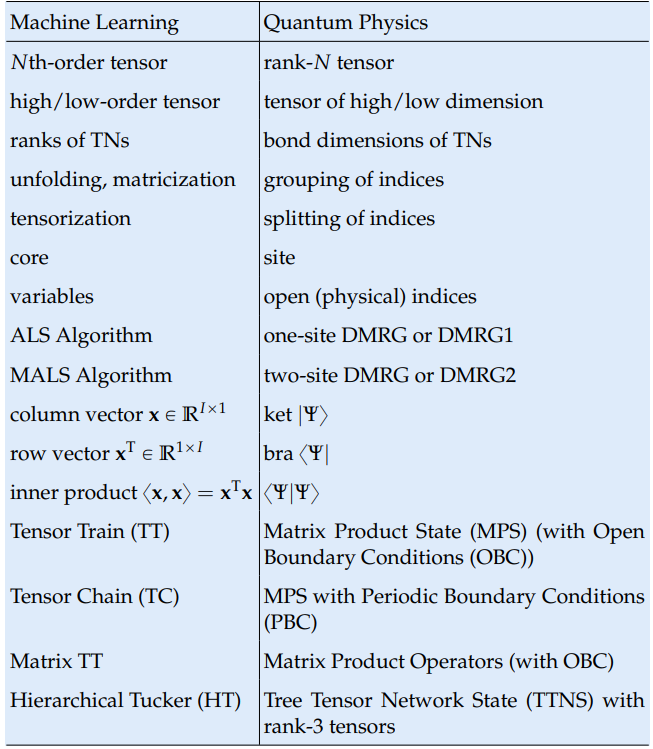
\includegraphics[width=0.6\textwidth]{lecture_10/figs/notation_diff.png}
\end{figure}
\end{frame}

%=======
\begin{frame}{Тензоры и графическое представление}
Определение 1. Под тензором $\tensor{A} \in \mathbb{F}^{I_1 \times ... \times I_d} $, $\mathbb{F} \in \{\mathbb{R}, \mathbb{C}\}$ будем понимать многомерный массив  с элементами $a_{i_1,...,i_d}$, где

$d$ --- размерность (иногда порядок или ранг),

$i_k$ --- размер k-ой моды

\begin{figure}
    \centering
    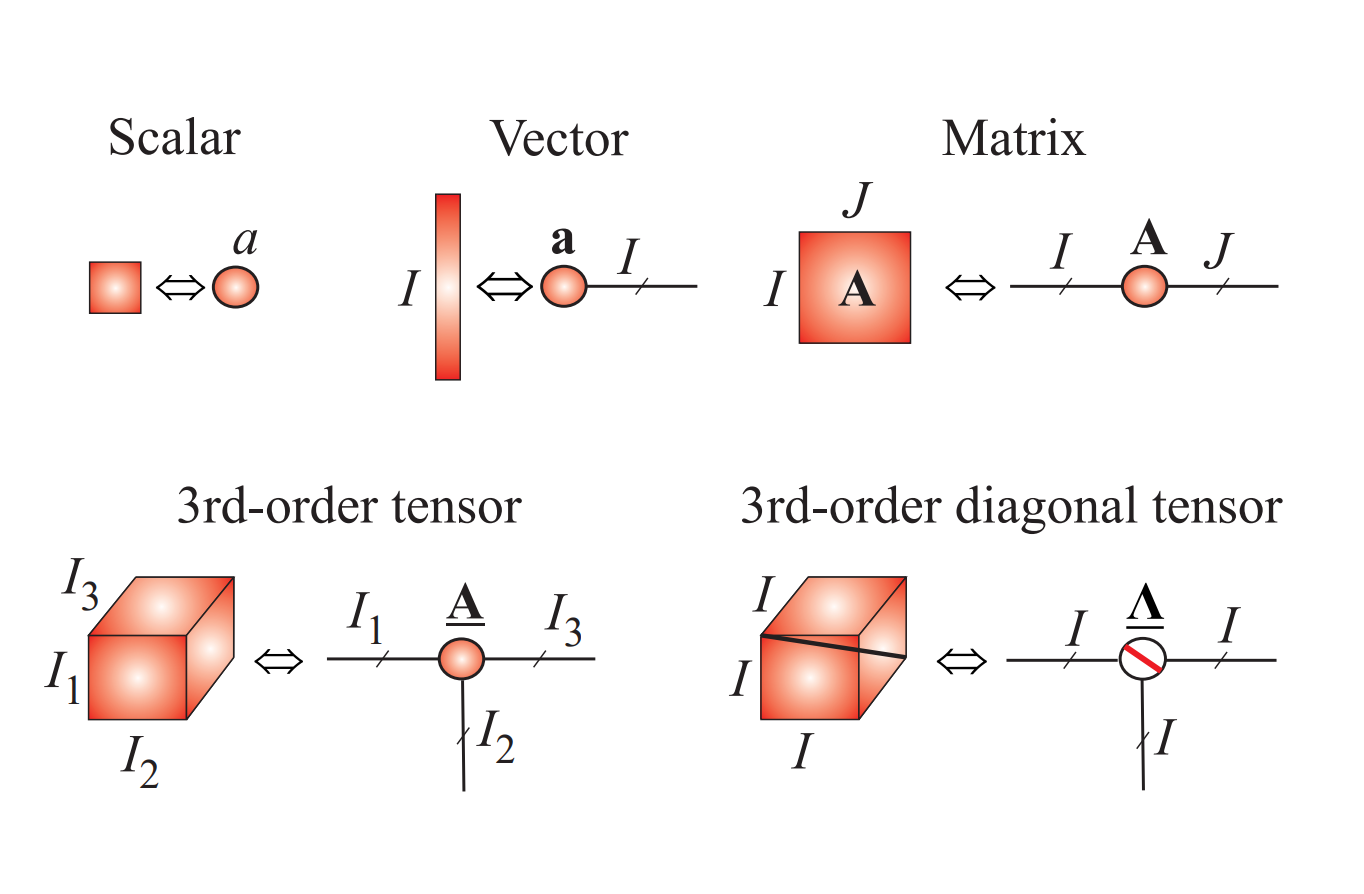
\includegraphics[width=0.8\textwidth]{lecture_10/figs/graph_repr_1.png}
\end{figure}
\end{frame}
%=======
\begin{frame}{Тензоры и графическое представление}
Определение 1. Под тензором $\tensor{A} \in \mathbb{F}^{I_1 \times ... \times I_d} $, $\mathbb{F} \in \{\mathbb{R}, \mathbb{C}\}$ будем понимать многомерный массив  с элементами $a_{i_1,...,i_d}$, где

$d$ --- размерность (иногда порядок или ранг),

$i_k$ --- размер k-ой моды

\begin{figure}
    \centering
    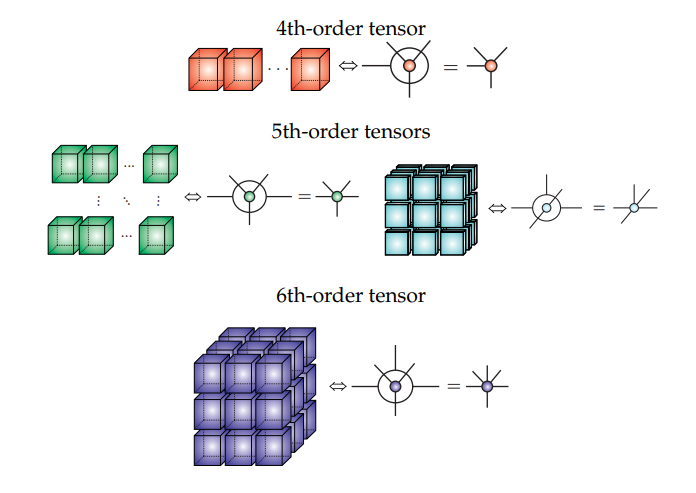
\includegraphics[width=0.8\textwidth]{lecture_10/figs/graph_repr_1_2.png}
\end{figure}
\end{frame}
%=======
\begin{frame}{Тензоры и графическое представление}
\begin{figure}
    \centering
    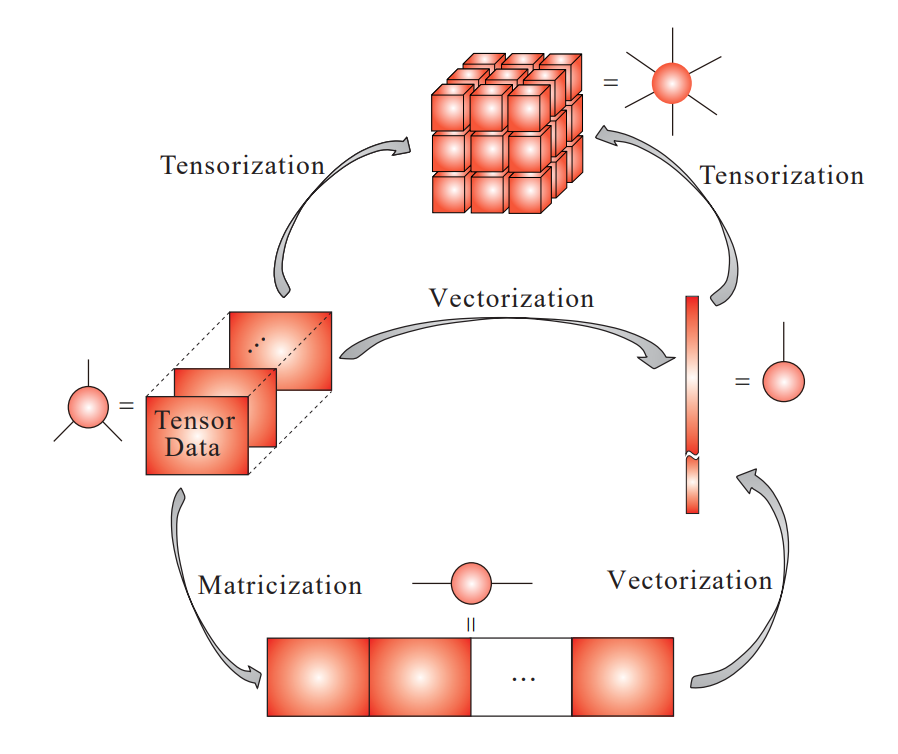
\includegraphics[width=0.7\textwidth]{lecture_10/figs/tensor_vector_matrix.png}
\end{figure}
\end{frame}
%=======
\begin{frame}{Тензоры и тензорные произведения}
Определение 2. Пусть есть два тензора $\tensor{A} \in \mathbb{R}^{I_1 \times ... \times I_d}$ $\tensor{B} \in \mathbb{R}^{J_1 \times ... \times J_D}$,  тогда назовём  их внешним произведением следующий тензор $\tensor{A} \circ \tensor{B} \in \mathbb{R}^{I_1 \times ... \times I_d \times J_1 \times ... \times J_D}$ с элементами:

$$(\tensor{A} \circ \tensor{B})_{i_1,...,i_d,j_1,...,j_D} = a_{i_1,...,i_d}b_{j_1,...,j_D}.$$

\end{frame}

%=======
\begin{frame}{Свёртка тензоров}

\begin{itemize}
    \item (N, 1)-свёртка (contraction) тензоров $\tensor{A} \in \mathbb{R}^{I_1 \times \dots \times I_N}$ и $\tensor{B} \in \mathbb{R}^{J_1 \times \dots \times J_M}$ (свёртка вдоль N-ой моды первого тензора и 1-ой моды второго), где обязательно $I_N = J_1$, даёт тензор 
    $\tensor{С} \in \mathbb{R}^{I_1 \times \dots \times I_{N-1} \times J_2 \times \dots \times J_M}$ с элементами:

    $$\tensor{C} = \tensor{A} \times_N^1 \tensor{B} = \tensor{A} \times^1 \tensor{B} = \tensor{A} \bullet \tensor{B}$$ 
    $$c_{i_1, ..., i_{N-1}, j_2, ..., j_M} = \sum_{i_N = 1}^{I_N} a_{i_1, ..., i_{N-1}, i_N} b_{i_N, j_2, ..., j_M}$$

    \item Можно также определить свёртку тензоров по нескольким индексам одновременно, например, так обозначается свёртка последних 3-ёх мод тензора $\tensor{A}$ и первых трёх мод тензора $\tensor{B}$ (операция требует совпадения соответствующих размерностей):
    $$\tensor{C} = \tensor{A} \times_{N, N-1, N-2}^{1, 2, 3} \tensor{B} $$ 
    $$c_{i_1, ..., i_{N-1}, j_2, ..., j_M} = \sum_{j_1 = 1}^{J_1}\sum_{j_2 = 1}^{J_2}\sum_{j_3 = 1}^{J_3} a_{i_1, ...,i_{N-3}, j_3, j_2, j_1} b_{j_1, j_2, j_3, ..., j_M}$$
\end{itemize}
    


\end{frame}
%=======

\begin{frame}{Свёртка тензоров}

Привычные операции над матрицами можно переписать и проиллюстрировать диаграммами как свёртки соответствующих тензоров:

\begin{figure}
    \centering
    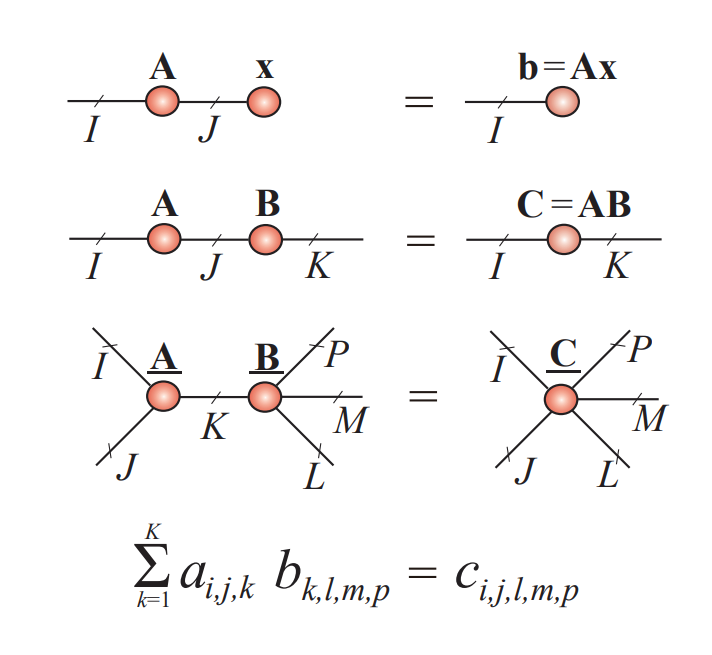
\includegraphics[width=0.6\textwidth]{lecture_10/figs/graph_repr_2.png}
\end{figure}
\end{frame}

%=======
\begin{frame}{Свёртка тензоров}
 Примеры свёрток тензоров более высокого порядка и свёрток по нескольким индексам одновременно:
\begin{figure}
    \centering
    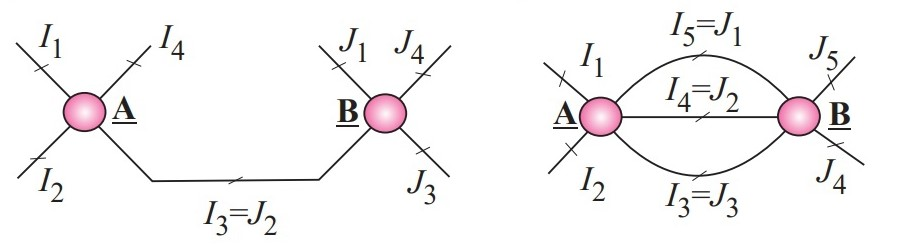
\includegraphics[width=0.9\textwidth]{lecture_10/figs/graph_repr_4.jpg}
\end{figure}

\begin{itemize}
    \item \textbf{Слева:} Свёртка двух тензоров 4-ого порядка вдоль 3-ей моды тензора  $\tensor{A}$ и 2-ой моды тензора $\tensor{B}$ даёт тензор 6-ого порядка $ \tensor{C} = \tensor{A} \times_3^2 \tensor{B} \in \mathbb{R}^{I_1 \times I_2 \times I_4 \times J_1 \times J_3 \times J_4}$ с элементами $c_{i_1, i_2, i_4, j_1, j_3, j_4} = \sum_{i_3} a_{i_1,i_2, i_3, i_4}b_{j_1, i_3, j_3,j_4}$.
    \item \textbf{Справа:} Свёртка двух тензоров 5-ого порядка вдоль мод 3,4, 5 тензора  $\tensor{A}$ и мод 1,2,3 тензора $\tensor{B}$ даёт тензор 4-ого порядка $ \tensor{C} = \tensor{A} \times_{5, 4, 3}^{1, 2, 3} \tensor{B} \in \mathbb{R}^{I_1 \times I_2  \times J_4 \times J_5}$.
    
\end{itemize}

\end{frame}

%=======
\begin{frame}{Свёртка тензоров}
\begin{figure}
    \centering
    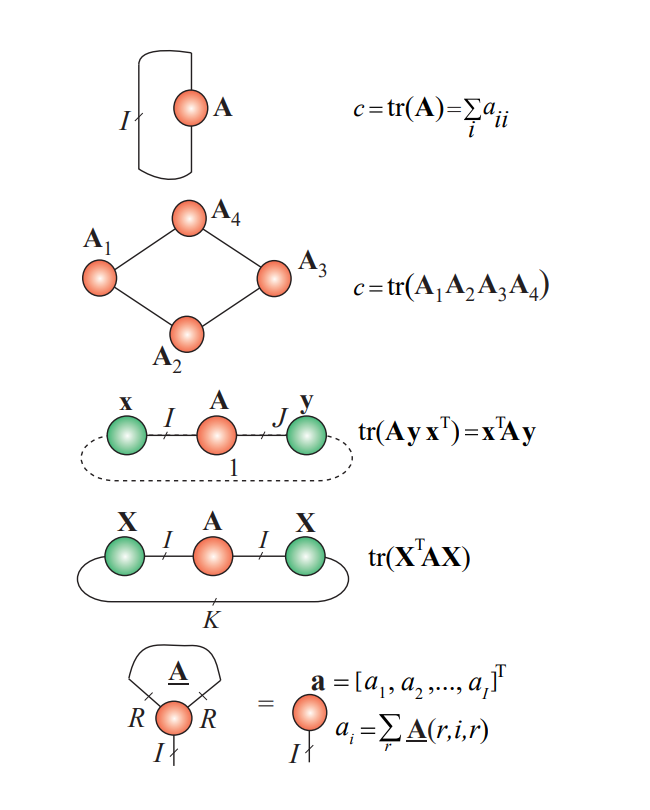
\includegraphics[width=0.6\textwidth]{lecture_10/figs/graph_repr_3.png}
\end{figure}
\end{frame}


%=======
\begin{frame}{Другие операции над тензорами}

\begin{itemize}
    \item Произведение $n$-ой моды тензора $\tensor{A} \in \mathbb{R}^{I_1 \times \dots \times I_N}$ и матрицы $\M{B} \in \mathbb{R}^{J \times I_n}$ даёт тензор $\tensor{С} \in \mathbb{R}^{I_1 \times \dots \times I_{n-1} \times J \times I_{n+1} \times \dots \times I_N}$ с элементами: $$\tensor{C} = \tensor{A} \times_n^2 \M{B} = \tensor{A} \times_n \M{B}, \quad  c_{i_1, ..., i_{n-1}, j, i_{n+1}, ..., i_N} = \sum_{i_n = 1}^{I_n} a_{i_1, ..., i_n, ..., i_N} b_{j,i_n}$$
    
    \item Мультилинейное произведение (произведение Такера) тензора $\tensor{G}$ и матриц $\M{B}^{(n)}$:

    $$ \tensor{C} = \big[ \tensor{G}; \M{B}^{(1)}, \dots, \M{B}^{(N)} \big] := \tensor{G} \times_1 \M{B}^{(1)} \times_2 \M{B}^{(2)} \times_3 \dots \times_N \M{B}^{(N)} $$

    \item Произведение $n$-ой моды тензора $\tensor{A} \in \mathbb{R}^{I_1 \times \dots \times I_N}$ и вектора $\M{b} \in \mathbb{R}^{I_n}$ даёт тензор $\tensor{С} \in \mathbb{R}^{I_1 \times \dots \times I_{n-1} \times I_{n+1} \times \dots \times I_N}$ с элементами:
    $$\tensor{C} = \tensor{A} \times_n^1 \M{b} =  \tensor{A} \bar{\times}_n \M{b}, \quad c_{i_1, ..., i_{n-1}, i_{n+1}, ..., i_N} = \sum_{i_n = 1}^{I_n} a_{i_1, ..., i_n, ..., i_N} b_{i_n}$$
    
\end{itemize}
\end{frame}
%=======
\begin{frame}{}
\begin{figure}
    \centering
    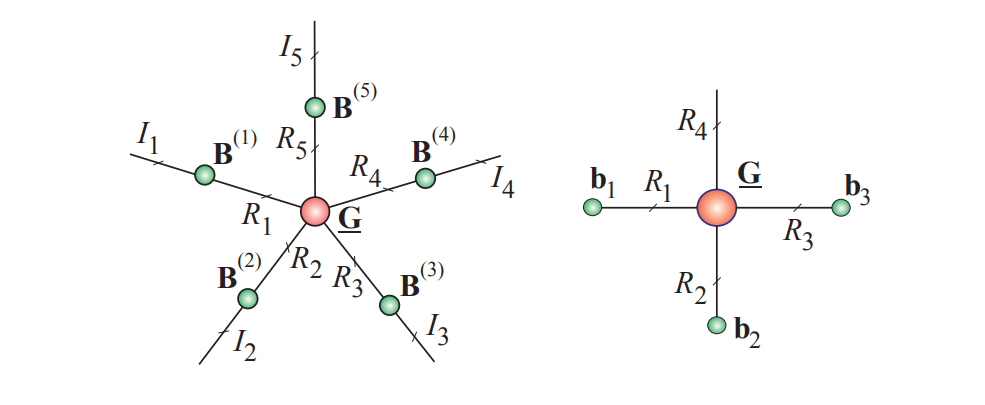
\includegraphics[width=\textwidth]{lecture_10/figs/G_BB_example.png}
\end{figure}

\begin{itemize}
    % \item[(a)] Трансформация/сжатие тензора 4-ого порядка $\tensor{G} \in \mathbb{R}^{R_1 \times R_2 \times R_3 \times R_4}$ в скаляр, вектор, матрицу и тензор 3-его порядка с помощью мультилинейного произведения тензора на векторы. Отметим, что произведение $n$-ой моды тензора на матрицу не меняет порядок тензора, а произведение этой моды на вектор уменьшает порядок на один. Например, мультилинейное произведение тензора 4-ого порядка и четырёх векторов даёт скаляр.
    \item \textbf{Слева:} Мультилинейное произведение тензора $\tensor{G} \in \mathbb{R}^{R_1 \times \dots \times R_5}$ и пяти матриц $\M{B}^{(n)} \in \mathbb{R}^{I_n \times R_n} \ (n = 1, \dots, 5)$ даёт тензор $ \tensor{C} = \big[ \tensor{G}; \M{B}^{(1)}, \dots, \M{B}^{(5)} \big] =$ \\
    $= \tensor{G} \times_1 \M{B}^{(1)} \times_2 \M{B}^{(2)} \times_3 \dots \times_5 \M{B}^{(5)} \in \mathbb{R}^{I_1 \times \dots \times I_5}$.
    \item \textbf{Справа:} Мультилинейное произведение тензора $\tensor{G} \in \mathbb{R}^{R_1 \times R_2 \times R_3 \times R_4}$ и трёх векторов $\M{b}_n \in \mathbb{R}^{R_n} \ (n = 1, 2, 3)$ даёт вектор $\M{c} = \tensor{G} \bar{\times}_1 \M{b}_1 \bar{\times}_2 \M{b}_2 \bar{\times}_3 \M{b}_3 \in \mathbb{R}^{R_4}$.
    
\end{itemize}
\end{frame}

%=======
\begin{frame}{Тензоры как мультилинейное отображение}
\begin{itemize}
    \item Напоминание из курса линейной алгебры: любой  матрице $\M{A} \in \mathbb{R}^{R_1 \times R_2}$ можно поставить в соответствие:
    \begin{enumerate}
        \item отображение из пространства $\mathbb{R}^{R_1}$ в пространство $\mathbb{R}^{R_2}$: $v \in \mathbb{R}^{R_1} \rightarrow Av \in \mathbb{R}^{R_2}$
        \item отображение из пространства $\mathbb{R}^{R_2}$ в пространство $\mathbb{R}^{R_1}$: $w \in \mathbb{R}^{R_2}\rightarrow A^Tw \in \mathbb{R}^{R_1}$
        \item билинейную функцию $(\cdot, \cdot)_{\M{A}}: \mathbb{R}^{R_1} \times \mathbb{R}^{R_2} \rightarrow \mathbb{R}$: $(v, w) \in \mathbb{R}^{R_1} \times \mathbb{R}^{R_2}  \rightarrow w^TAv \in \mathbb{R}$
    \end{enumerate}
    \item По аналогии, тензору $\tensor{A} \in \mathbb{R}^{I_1 \times \dots \times I_N}$ порядка $N$ можно сопоставлять различные отображения с помощью операции произведения Такера (мультилинейного произведения), например:
    \begin{itemize}
        \item[$\blacksquare$] отображение из $\mathbb{R}^{I_2} \times \dots \times \mathbb{R}^{I_N}$ в $\mathbb{R}^{I_1}:$

        $$(v^{(2)}, \dots, v^{(N)}) \rightarrow \big[ \tensor{A}; I, v^{(2)}, \dots, v^{(N)} \big] \in \mathbb{R}^{I_1}$$
    \end{itemize}
    \item Таким образом для тензоров можно определить понятия нормы, сингулярных чисел и т.д. (будет рассмотрено подробнее в дальнейшем).
\end{itemize}
\end{frame}
%=======
\begin{frame}{Пример 1. HOPLS}
\begin{figure}
    \centering
    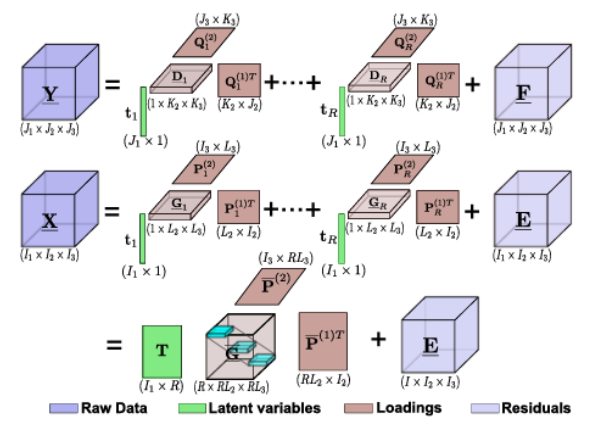
\includegraphics[width=0.6\textwidth]{lecture_10/figs/HOPLS.png}
\end{figure}
\begin{figure}
    \centering
    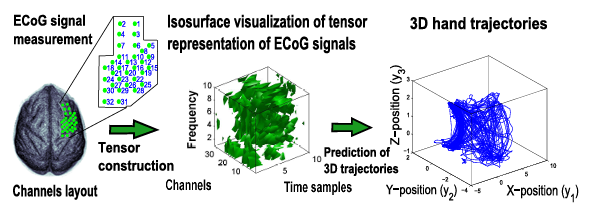
\includegraphics[width=0.6\textwidth]{lecture_10/figs/HOPLS_example.png}
\end{figure}

\end{frame}
%=======
\begin{frame}{Пример 1. Tucker decompositions}
\begin{figure}
    \centering
    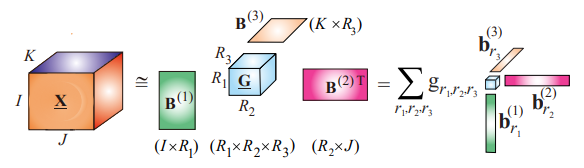
\includegraphics[width=0.6\textwidth]{lecture_10/figs/Tucker_decompositions.png}
\end{figure}
\begin{figure}
    \centering
    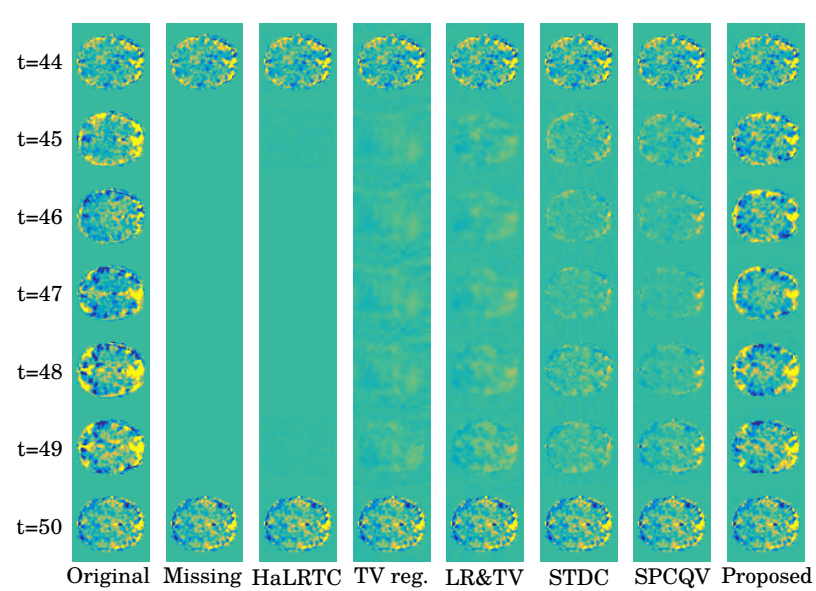
\includegraphics[width=0.6\textwidth]{lecture_10/figs/Tucker_decompositions_example.png}
\end{figure}
\end{frame}
% %=======
% \begin{frame}{Резюме}
% \begin{itemize}
%     \item 123
% \end{itemize}
% \end{frame}
\end{document} 